%# -*- coding: utf-8-unix -*-
%%==================================================
%% chapter01.tex for SJTU Master Thesis
%%==================================================

%\bibliographystyle{sjtu2}%[此处用于每章都生产参考文献]

\chapter{绪论}
\label{chap:introduction}

现代社会地理位置获取和移动计算科技进步,促使轨迹数据的大规模发展。这些轨迹数据体现了例如人类,车辆以及动物等移动物体的移动多样性。在过去十几年间,许多旨在处理、管理和挖掘轨迹数据的算法与技术许多应用中有着广泛而重要的应用价值。如今以轨迹数据挖掘为首的轨迹数据处理技术已经日趋系统规范,从轨技数据生成,轨技数据预处理,到轨技数据管理,再到多样的数据挖掘任务(例如轨迹模式挖掘、轨迹异常检测、轨迹分类等等)。已有轨迹处理和轨迹挖掘的技术在相互应用中有着重要的联系与关联,轨迹数据转化成其他轨迹形式,例如图、矩阵和张量的方法也在越来越多的轨迹数据挖掘和机器学习领域有着常见的应用。

轨迹从概念上定义是一个移动物体的移动轨迹,轨迹数据可以用于许多领域的复杂分析。例如,公共交通系统可以应用过去时刻的轨迹数据分析交通流量模式并找出致使交通拥塞的原因;生物领域的动物长途迁移轨迹或是短途移动变化可以为人类提供宝贵的数据分析人类活动对生态环境的影响程度;还可以通过分析数据预测城乡车辆移动情况并及时提供符合公众出行的公共交通支持。其他应用领域也包括了路径优化设计,公共交通安全管理和基于兴趣点的用户个性化服务。

基于以上应用情景,轨迹数据挖掘在计算机科学、社会学和地理学领域都变得愈发重要。在轨技数据挖掘领域研究从深度和广度都已经取得了不错的成果,从图\ref{fig:SRR}可以看出当前轨迹数据挖掘与处理的基本研究步骤。本课题相似轨迹查询方法设计与实现主要基于其该范例中的轨迹预处理与轨迹数据索引与获取这两个领域中已存在的方法,并结合自己的理解和数据的格式实现改善和创新。
\\
\begin{figure}[!htp]
  \centering
  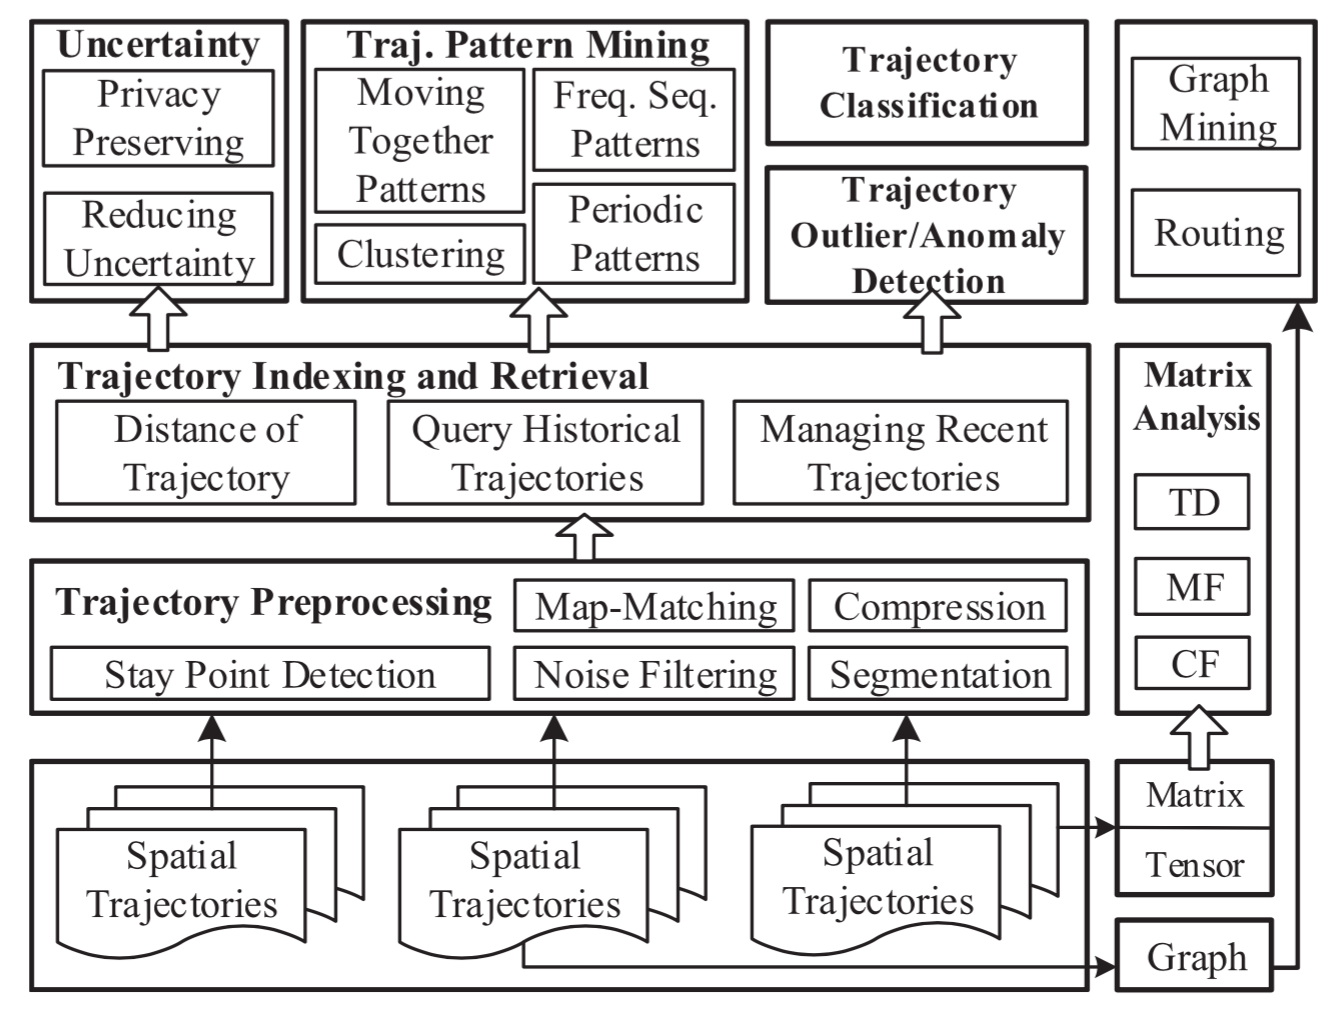
\includegraphics[width=0.9\textwidth]{chapter01/paradigm.png}
  \bicaption[fig:SRR]{这里将出现在插图索引中}{轨技数据挖掘范例}{Fig}{Paradigm of trajectory data mining}
\end{figure}


\section{相似轨迹查询}
\label{sec:requirements}
大量空间轨迹数据为我们提供了分析移动物体移动方式的可能性,这种移动方式的分析可以体现出单个轨迹所包含的某种特定移动方式或是一组轨迹所共享的相似移动方式。

\subsection{轨迹查询概念简介}
\label{sec:requirements}

完成在轨迹数据库中复杂的轨迹查询操作是复杂且费时的操作,因为轨迹数据库的规模一般是非常庞大的。因此,轨迹数据库的一个重要点事支持高效的轨迹索引以加速轨迹插叙过程。通常情况下,时空数据的索引技术是空间数据索引辅以时间度量参数。轨迹查询既关注经过的地理位置的拓扑位置顺序,也关注空间物体之间的距离度量,从简单的欧式距离度量到复杂的轨迹之间相似性。从大体上说,如今的轨迹查询依照时空关系分为三类:1)$P$-$query$,查询满足特定轨迹段或者时空关系的兴趣点或者查询针对某些兴趣点满足时空关系的轨迹;2)$R$-$query$,根据给定的时空区域查询轨迹或者给定轨迹查询目的区域,3)$T$-$query$, 查询在一组轨迹数据集中查询相似轨迹或在给定的距离阈值内查询轨迹。


\subsection{相似轨迹查询应用现状}
\label{sec:requirements}

\subsection{相似轨迹查询方法设计}
\label{sec:requirements}

\section{论文大致结构}
\label{sec:requirements}

\section{本章小结}
\label{sec:requirements}


